\documentclass[
    author={Jacob Daniel Halsey},
    supervisor={Prof. Awais Rashid},
    degree={BSc},
    title={Building a Testbed for Evaluating Privacy Enhancing Technologies  (PETs)},
    subtitle={},
    type={software development},
    year={2021}
]{dissertation}

\usepackage[backend=biber,bibstyle=ieee,citestyle=numeric]{biblatex}
\bibliography{dissertation}

\usepackage{setspace} 
\setstretch{1.25}

\usepackage{subfig}

\begin{document}

\maketitle
\frontmatter
\makedecl
\tableofcontents

\chapter*{Executive Summary}

The goal of this project is to produce a simple and lightweight testbed platform for evaluating privacy enhancing
technologies.
It should provide support for testing varied architectures and network topologies, such as client-server and
peer-to-peer applications.
It should also support simulating applications for different types of platforms including mobile phone apps.

\vspace{1cm}

Summary of work:

\begin{itemize}
\item I have developed a flexible command line tool called \emph{kvm-compose} for Linux using the Rust
      language and \emph{libvirt} library for building and destroying virtual testing environments.
\item In the process I have made some contributions to the \emph{libvirt-rust} language
      bindings open source library.
\item I have then implemented some example projects using the testbed tool.
\end{itemize}

\chapter*{Supporting Technologies}

\begin{singlespace}
	\begin{itemize}
		\item \emph{Linux KVM} (Kernel-based Virtual Machine) - \url{https://www.linux-kvm.org/}
		\item \emph{Open vSwitch} Virtual multilayer switch - \url{https://www.openvswitch.org/}
		\item \emph{libvirt} Virtualization API - \url{https://libvirt.org/}
		\item \emph{Rust} Language, Compiler, Toolchain, etc. - \url{https://www.rust-lang.org/}
		\item \emph{libvirt-rust} Rust bindings to the libvirt - \url{https://gitlab.com/libvirt/libvirt-rust}
		\item \emph{clap} Rust command Line Argument Parser - \url{https://github.com/clap-rs/clap}
		\item \emph{serde} Rust Serialization framework - \url{https://github.com/serde-rs/}
		\item \emph{serde-yaml} YAML backend for serde - \url{https://github.com/dtolnay/serde-yaml}
		\item \emph{serde-plain} Plain text backend for serde - \url{https://github.com/mitsuhiko/serde-plain}
		\item \emph{thiserror} Rust error derive macro - \url{https://github.com/dtolnay/thiserror}
		\item \emph{anyhow} Rust error handling framework - \url{https://github.com/dtolnay/anyhow}
		\item \emph{simple\_logger} Rust logging implementation - \url{https://github.com/borntyping/rust-simple_logger}
		\item \emph{xml-rs} XML library for Rust - \url{https://github.com/netvl/xml-rs}
		\item \emph{validator} Rust struct validation - \url{https://github.com/Keats/validator}
		\item \emph{directories} User data directories library - \url{https://github.com/dirs-dev/directories-rs}
		\item \emph{reqwest} Rust HTTP Client - \url{https://github.com/seanmonstar/reqwest}
		\item \emph{indicatif} Rust command line progress indicator - \url{https://github.com/mitsuhiko/indicatif}
		\item \emph{tempfile} Rust temporary file library - \url{https://github.com/Stebalien/tempfile}
		\item \emph{casual} Rust user input parser - \url{https://github.com/rossmacarthur/casual}
		\item \emph{derive-new} Rust new constructor macro - \url{https://github.com/nrc/derive-new}
		\item \emph{enum-iterator} Rust macro for iterating enums - \url{https://github.com/stephaneyfx/enum-iterator}
		\item \emph{rust-embed} Embeds files into Rust binaries - \url{https://github.com/pyros2097/rust-embed}
	\end{itemize}
\end{singlespace}

\chapter*{Acknowledgements}

I would like to thank my supervisor Professor Awais Rashid and co-supervisor Joe Gardiner for their
project proposal and support and guidance in completing it.

\mainmatter


\chapter{Contextual Background}
\label{chap:context}

The UK Research and Innovation (UKRI) is a non-departmental public body of the United Kingdom Government
sponsored by the Department for Business, Energy and Industrial Strategy~\cite{ukri_who_we_are}.
In October 2020 the UKRI announced the creation of the National Research Centre on Privacy, Harm Reduction
and Adversarial Influence Online (REPHRAIN)~\cite{ukri_new_centre}.
The centre is made up of researchers in computer science, international relations, law, psychology, management,
design, digital humanities, public policy, political Science, criminology, and sociology from five British
universities including the University of Bristol. \\

REPHRAIN should be understood in the context of the UK government's \emph{Online Harms White Paper} public
consultation beginning in April 2019~\cite{uk_gov_online_harms}, which sets out plans for new online safety 
measures; REPHRAIN's missions and outcomes are aligned with this paper~\cite{rephrain_harms}. \\

REPHRAIN will focus on three core missions~\cite{rephrain_missions}:

\begin{enumerate}
	\item Delivering privacy at scale while mitigating its misuse to inflict harms.
	\item Minimising harms while maximising benefits from a sharing-driven digital economy.
	\item Balancing individual agency vs. the social good.
\end{enumerate}

The three missions will require looking at Privacy Enhancing Technologies (PETs); including their capabilities,
applications of PETs in addressing existing online harms, mitigating the potential abuse of PETs, embedding the PETs
into infrastructures, and developing new PETs.
In order to facilitate this REPHRAIN intends to build a toolbox of resources including a PETs testbed. The testbed
will be used researchers in developing, testing, and evaluating the PETs. The aim of this project is to develop
a prototype for this testbed.

\section{What are Privacy Enhancing Technologies (PETs)?}

Before we discuss Privacy Enhancing Technologies we must consider what we mean by "privacy". REPHRAIN is 
primarily using the definitions set out by D. J. Solove in his
2006 article \emph{A Taxonomy of Privacy}~\cites{solove_privacy}{rephrain_harms}. Solove notes that the
definition of privacy has often been very broad or vague, and therefore sets out to develop
a taxonomy of privacy violations. He has defined four groups of harmful activities (See figure \ref{privacy_taxonomy}). \\

\begin{figure}
\centering
\parbox{7cm}{
	\begin{enumerate}
		\item Information collection
		\begin{enumerate}
			\item Surveillance
			\item Interrogation 
		\end{enumerate}
		\item Information processing
		\begin{enumerate}
			\item Aggregation
			\item Identification
			\item Insecurity
			\item Secondary Use
			\item Exclusion
		\end{enumerate}
	\end{enumerate}
}
\qquad
	\begin{minipage}{7cm}
		\begin{enumerate}
			\setcounter{enumi}{2}
			\item Information  dissemination
			\begin{enumerate}
				\item Breach of Confidentiality
				\item Disclosure
				\item Exposure
				\item Increased Accessibility
				\item Blackmail
				\item Appropriation
				\item Distortion
			\end{enumerate}
			\item Invasion
			\begin{enumerate}
				\item Intrusion
				\item Decisional Interference
			\end{enumerate} 
		\end{enumerate}
	\end{minipage}
	\caption{A Taxonomy of Privacy Violations~\cite{solove_privacy}.}
	\label{privacy_taxonomy}
\end{figure}

Broadly speaking a Privacy Enhancing Technology is any solution or approach in hardware or software that helps
protect a user from such privacy violations~\cite{buckley_pets}. Some examples of PETs could include 
Onion routing such as the Tor network (which enables anonymous communication), or
end-to-end encrypted messaging systems such as the Signal protocol. 
Kaaniche et al. \cite{kaaniche_2020_privacy} have defined a more comprehensive classification of PETs
 (see Figure \ref{pet_taxonomy}).

\begin{figure}
	\centering
	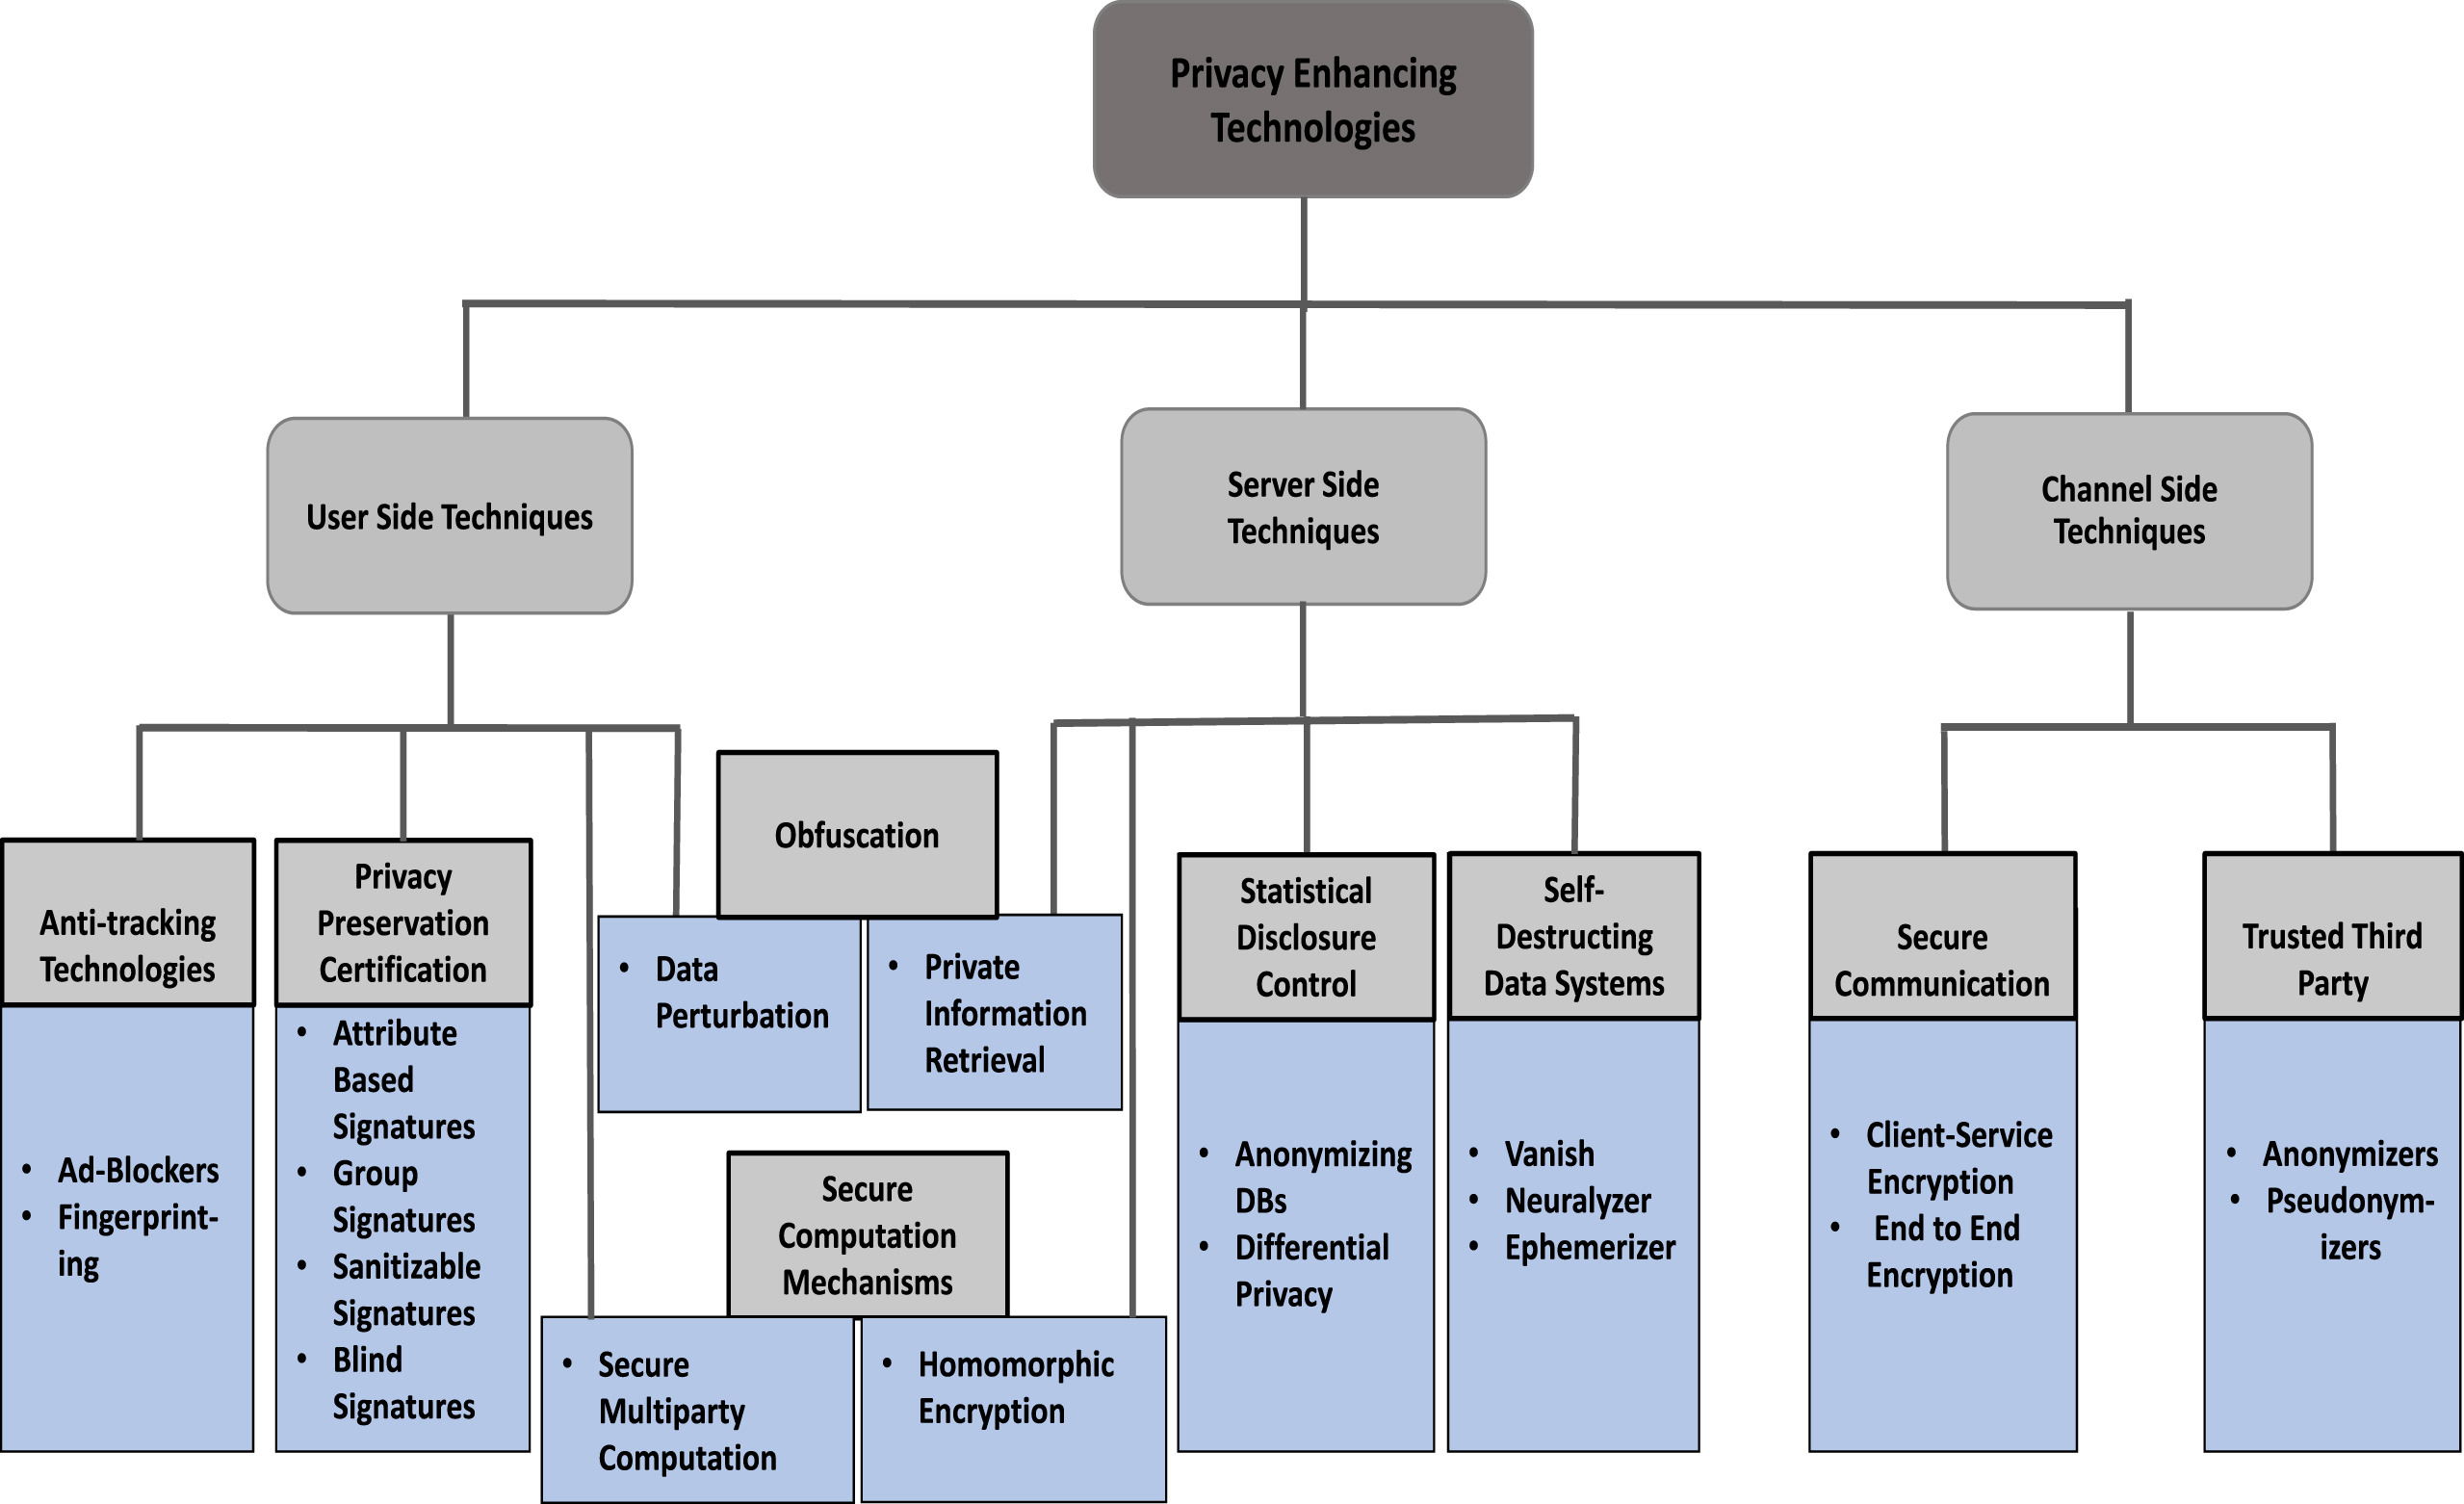
\includegraphics{img/pet_taxonomy}
	\caption{A Taxonomy of privacy enhancing technologies~\cite{kaaniche_2020_privacy}.}
	\label{pet_taxonomy}
\end{figure}

\section{Existing Solutions}

There has been some existing research by Tekeoglu and Tosun~\cite{tekeoglu_2016_testbed} who have developed 
a privacy testbed for Internet-of-Things (IoT) devices. Their approach has some similar goals to this project 
in that it looks at capturing layer 2 and 3 network traffic. They note that the testbed enables experiments such
as port vulnerability scans, checking what cipher suites are used (or not), and generally monitoring 
network traffic to see what data is being collected. However their testbed is different in that it is only designed
for IoT devices; rather than general purpose PET applications.

\section{High Level Objectives}

Overall the high-level objective of this project is to develop a simple and lightweight
testbed platform for evaluating PETs:

\begin{itemize}
	\item The testbed should support testing various architectures and network topologies, 
	including client/server and peer-to-peer applications, to accommodate a variety of PETs.
	\item The testbed must be able to collect information such as packet captures
	for use in evaluating the privacy properties.
	\item The testbed should support different platforms such as desktop and mobile apps,
	and both applications where the source code is available or only pre-built binaries.
	\item The testbed should enable a high level of automation, such that working with large test
	environments because feasible, and the setup can easily and programmatically be replicated.
\end{itemize}

\chapter{Technical Background}
\label{chap:technical}

{\bf A compulsory chapter,     of roughly $10$ pages} 
\vspace{1cm} 

\noindent
This chapter is intended to describe the technical basis on which execution
of the project depends.  The goal is to provide a detailed explanation of
the specific problem at hand, and existing work that is relevant (e.g., an
existing algorithm that you use, alternative solutions proposed, supporting
technologies).  

Per the same advice in the handbook, note there is a subtly difference from
this and a full-blown literature review (or survey).  The latter might try
to capture and organise (e.g., categorise somehow) {\em all} related work,
potentially offering meta-analysis, whereas here the goal is simple to
ensure the dissertation is self-contained.  Put another way, after reading 
this chapter a non-expert reader should have obtained enough background to 
understand what {\em you} have done (by reading subsequent sections), then 
accurately assess your work.  You might view an additional goal as giving 
the reader confidence that you are able to absorb, understand and clearly 
communicate highly technical material.

\chapter{Project Execution}
\label{chap:execution}

{\bf A topic-specific chapter, of roughly $15$ pages} 
\vspace{1cm} 

\noindent
This chapter is intended to describe what you did: the goal is to explain
the main activity or activities, of any type, which constituted your work 
during the project.  The content is highly topic-specific, but for many 
projects it will make sense to split the chapter into two sections: one 
will discuss the design of something (e.g., some hardware or software, or 
an algorithm, or experiment), including any rationale or decisions made, 
and the other will discuss how this design was realised via some form of 
implementation.  

This is, of course, far from ideal for {\em many} project topics.  Some
situations which clearly require a different approach include:

\begin{itemize}
\item In a project where asymptotic analysis of some algorithm is the goal,
      there is no real ``design and implementation'' in a traditional sense
      even though the activity of analysis is clearly within the remit of
      this chapter.
\item In a project where analysis of some results is as major, or a more
      major goal than the implementation that produced them, it might be
      sensible to merge this chapter with the next one: the main activity 
      is such that discussion of the results cannot be viewed separately.
\end{itemize}

\noindent
Note that it is common to include evidence of ``best practice'' project 
management (e.g., use of version control, choice of programming language 
and so on).  Rather than simply a rote list, make sure any such content 
is useful and/or informative in some way: for example, if there was a 
decision to be made then explain the trade-offs and implications 
involved.

\section{Example Section}

This is an example section; 
the following content is auto-generated dummy text.
\lipsum

\subsection{Example Sub-section}

\begin{figure}[t]
\centering
foo
\caption{This is an example figure.}
\label{fig}
\end{figure}

\begin{table}[t]
\centering
\begin{tabular}{|cc|c|}
\hline
foo      & bar      & baz      \\
\hline
$0     $ & $0     $ & $0     $ \\
$1     $ & $1     $ & $1     $ \\
$\vdots$ & $\vdots$ & $\vdots$ \\
$9     $ & $9     $ & $9     $ \\
\hline
\end{tabular}
\caption{This is an example table.}
\label{tab}
\end{table}

\begin{algorithm}[t]
\For{$i=0$ {\bf upto} $n$}{
  $t_i \leftarrow 0$\;
}
\caption{This is an example algorithm.}
\label{alg}
\end{algorithm}

\begin{lstlisting}[float={t},caption={This is an example listing.},label={lst},language=C]
for( i = 0; i < n; i++ ) {
  t[ i ] = 0;
}
\end{lstlisting}

This is an example sub-section;
the following content is auto-generated dummy text.
Notice the examples in Figure~\ref{fig}, Table~\ref{tab}, Algorithm~\ref{alg}
and Listing~\ref{lst}.
\lipsum

\subsubsection{Example Sub-sub-section}

This is an example sub-sub-section;
the following content is auto-generated dummy text.
\lipsum

\paragraph{Example paragraph.}

This is an example paragraph; note the trailing full-stop in the title,
which is intended to ensure it does not run into the text.

\chapter{Critical Evaluation}
\label{chap:evaluation}

{\bf A topic-specific chapter, of roughly $15$ pages} 
\vspace{1cm} 

\noindent
This chapter is intended to evaluate what you did.  The content is highly 
topic-specific, but for many projects will have flavours of the following:

\begin{enumerate}
\item functional  testing, including analysis and explanation of failure 
      cases,
\item behavioural testing, often including analysis of any results that 
      draw some form of conclusion wrt. the aims and objectives,
      and
\item evaluation of options and decisions within the project, and/or a
      comparison with alternatives.
\end{enumerate}

\noindent
This chapter often acts to differentiate project quality: even if the work
completed is of a high technical quality, critical yet objective evaluation 
and comparison of the outcomes is crucial.  In essence, the reader wants to
learn something, so the worst examples amount to simple statements of fact 
(e.g., ``graph X shows the result is Y''); the best examples are analytical 
and exploratory (e.g., ``graph X shows the result is Y, which means Z; this 
contradicts [1], which may be because I use a different assumption'').  As 
such, both positive {\em and} negative outcomes are valid {\em if} presented 
in a suitable manner.

\chapter{Conclusion}
\label{chap:conclusion}

{\bf A compulsory chapter,     of roughly $5$ pages} 
\vspace{1cm} 

\noindent
The concluding chapter of a dissertation is often underutilised because it 
is too often left too close to the deadline: it is important to allocation
enough attention.  Ideally, the chapter will consist of three parts:

\begin{enumerate}
\item (Re)summarise the main contributions and achievements, in essence
      summing up the content.
\item Clearly state the current project status (e.g., ``X is working, Y 
      is not'') and evaluate what has been achieved with respect to the 
      initial aims and objectives (e.g., ``I completed aim X outlined 
      previously, the evidence for this is within Chapter Y'').  There 
      is no problem including aims which were not completed, but it is 
      important to evaluate and/or justify why this is the case.
\item Outline any open problems or future plans.  Rather than treat this
      only as an exercise in what you {\em could} have done given more 
      time, try to focus on any unexplored options or interesting outcomes
      (e.g., ``my experiment for X gave counter-intuitive results, this 
      could be because Y and would form an interesting area for further 
      study'' or ``users found feature Z of my software difficult to use,
      which is obvious in hindsight but not during at design stage; to 
      resolve this, I could clearly apply the technique of Smith [7]'').
\end{enumerate}

\backmatter
\printbibliography

\end{document}
